\documentclass[xcolor=svgnames]{beamer}
\usepackage[utf8]{inputenc}
\usepackage[english]{babel}

\usetheme{Proso}

\title{Interactive Machine Learning}
\author{Jan Papoušek}
\institute{Masaryk University Brno}
\date{\today}

\begin{document}
% --------------------------- SLIDE --------------------------------------------
\frame[plain]{\titlepage}
% ------------------------------------------------------------------------------
% --------------------------- SLIDE --------------------------------------------
\begin{frame}
	\frametitle{Classical Machine Learning}
	\begin{center}
		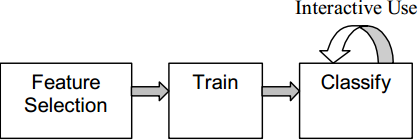
\includegraphics[width=.75\textwidth]{img/cml.png}
	\end{center}
\end{frame}
% ------------------------------------------------------------------------------
% --------------------------- SLIDE --------------------------------------------
\begin{frame}
	\frametitle{Classical Machine Learning}
	\begin{itemize}
		\item relatively few carefully chosen features
		\item limited training data
		\item classifier must amplify that limited training data
					into excellent performance on new data
		\item time to train the classifier is relatively unimportant as
					long as it does not take too many days
	\end{itemize}
\end{frame}
% ------------------------------------------------------------------------------
% --------------------------- SLIDE --------------------------------------------
\begin{frame}
	\frametitle{Interactive Machine Learning}
	\begin{center}
		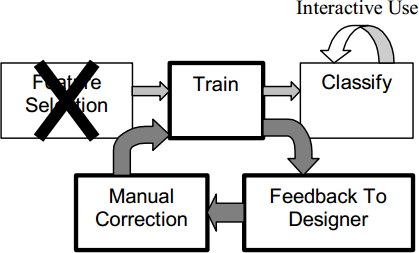
\includegraphics[width=.75\textwidth]{img/iml.png}
	\end{center}
\end{frame}
% ------------------------------------------------------------------------------
% --------------------------- SLIDE --------------------------------------------
\begin{frame}
	\frametitle{Interactive Machine Learning}
	\begin{itemize}
		\item learn/train very quickly
		\item accommodate 100s to 1000s of features
		\item	perform feature selection
		\item allow for tens to hundreds of thousands of training examples
	\end{itemize}
\end{frame}
% ------------------------------------------------------------------------------
% --------------------------- SLIDE --------------------------------------------
\begin{frame}
	\begin{center}
		{\Huge Interactive Machine Learning}

		\medskip
		human teaches machine

		\bigskip
		\bigskip
		\bigskip
		\bigskip

		{\Huge Education}

		\medskip
		machine teaches human
	\end{center}
\end{frame}
% ------------------------------------------------------------------------------
% --------------------------- SLIDE --------------------------------------------
\begin{frame}
	\frametitle{Case Study -- Crayons}
	\begin{center}
		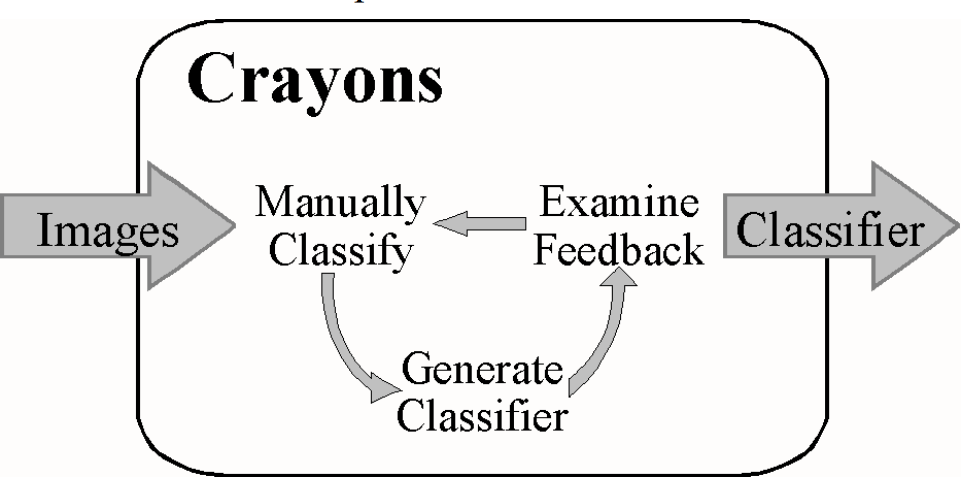
\includegraphics[width=0.75\textwidth]{img/crayons-diagram.png}
	\end{center}
\end{frame}
% ------------------------------------------------------------------------------
% --------------------------- SLIDE --------------------------------------------
\begin{frame}
	\frametitle{Case Study -- Crayons}
	\begin{center}
		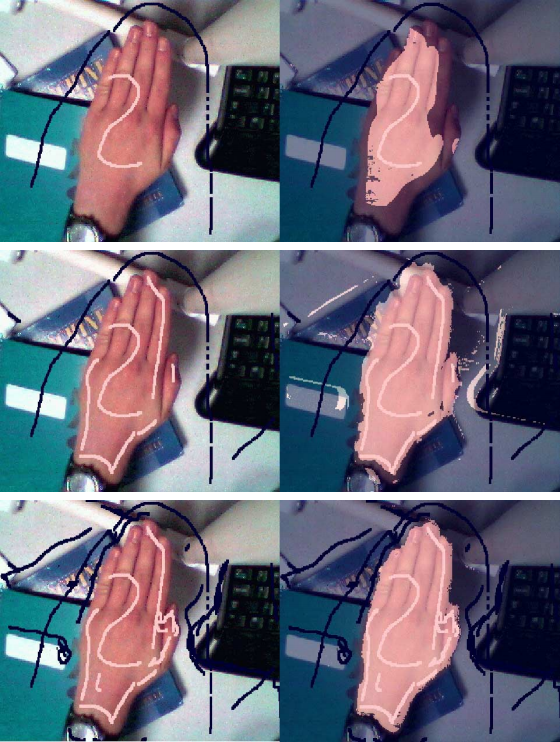
\includegraphics[width=0.5\textwidth]{img/crayons-example.png}
	\end{center}
\end{frame}
% ------------------------------------------------------------------------------
% --------------------------- SLIDE --------------------------------------------
\begin{frame}
	\frametitle{Case Study -- Crayons}
	\begin{center}
		{\Large decision trees}
	\end{center}

	\begin{itemize}
		\item DT algorithm leads to the feature selection
		\item two strategies:
			\begin{itemize}
				\item center weighted (CW) -- slower, better classifiers
				\item mean split (MS) -- faster, worse classifiers
			\end{itemize}
	\end{itemize}
\end{frame}
% ------------------------------------------------------------------------------
% --------------------------- SLIDE --------------------------------------------
\begin{frame}
	\frametitle{Case Study -- Crayons}
	\begin{columns}
		\column{.5\textwidth}
		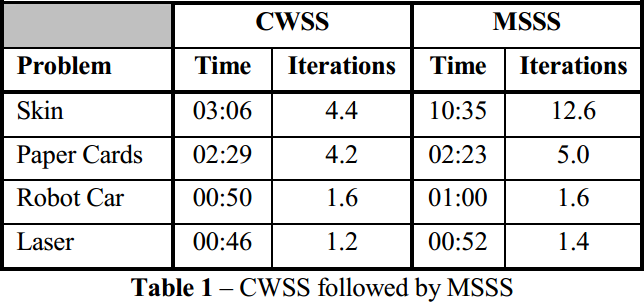
\includegraphics[width=\textwidth]{img/crayons-cwss-msss.png}
		\column{.5\textwidth}
		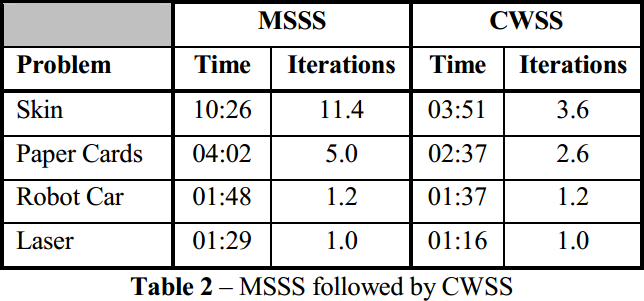
\includegraphics[width=\textwidth]{img/crayons-msss-cwss.png}
	\end{columns}
\end{frame}
% ------------------------------------------------------------------------------
% --------------------------- SLIDE --------------------------------------------
\begin{frame}
	\frametitle{Case Study -- Crayons}
	\begin{center}
		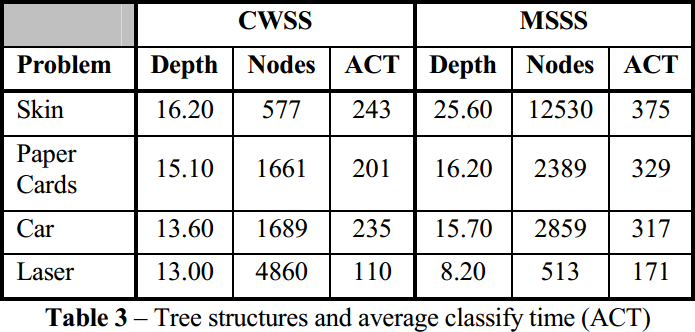
\includegraphics[width=\textwidth]{img/crayons-results.png}
	\end{center}
\end{frame}
% ------------------------------------------------------------------------------
% --------------------------- SLIDE --------------------------------------------
\begin{frame}
	\frametitle{Case Study -- PBC System}
	\begin{center}
		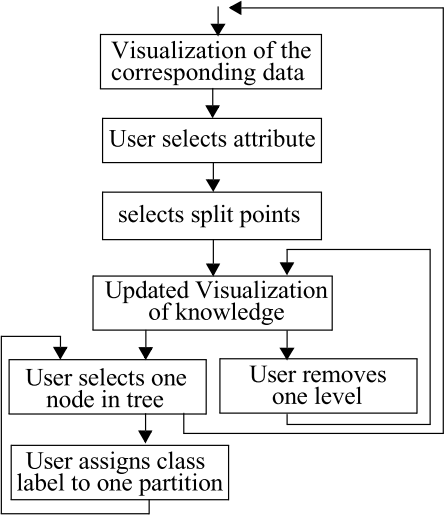
\includegraphics[width=0.5\textwidth]{img/pbc-diagram.png}
	\end{center}
\end{frame}
% ------------------------------------------------------------------------------
% --------------------------- SLIDE --------------------------------------------
\begin{frame}
	\frametitle{Case Study -- PBC System}
	\begin{center}
		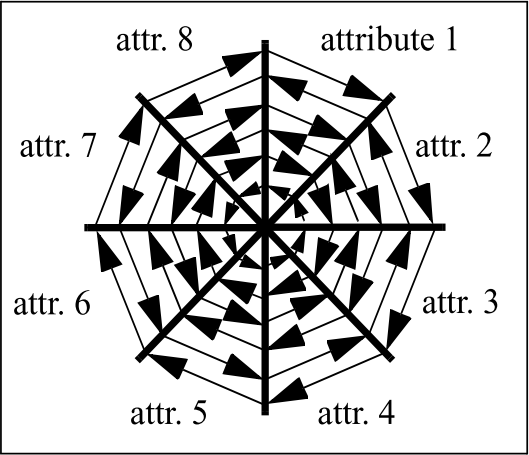
\includegraphics[width=0.75\textwidth]{img/pbc-circle-segments.png}
	\end{center}
\end{frame}
% ------------------------------------------------------------------------------
% --------------------------- SLIDE --------------------------------------------
\begin{frame}
	\frametitle{Case Study -- PBC System}
	\begin{center}
		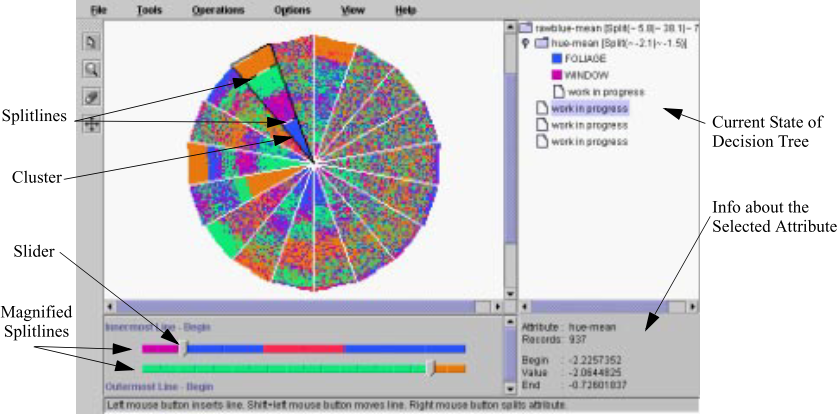
\includegraphics[width=0.95\textwidth]{img/pbc-screenshot.png}
	\end{center}
\end{frame}
% ------------------------------------------------------------------------------
% --------------------------- SLIDE --------------------------------------------
\begin{frame}
	\frametitle{Case Study -- PBC System}
	\begin{center}
		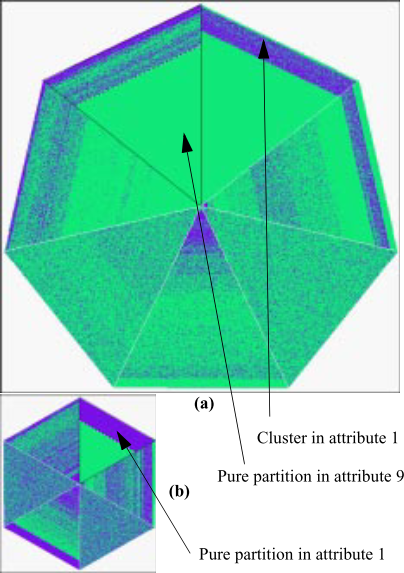
\includegraphics[width=0.45\textwidth]{img/pbc-example.png}
	\end{center}
\end{frame}
% ------------------------------------------------------------------------------
% --------------------------- SLIDE --------------------------------------------
\begin{frame}
	\frametitle{Case Study -- PBC System}
	\begin{center}
		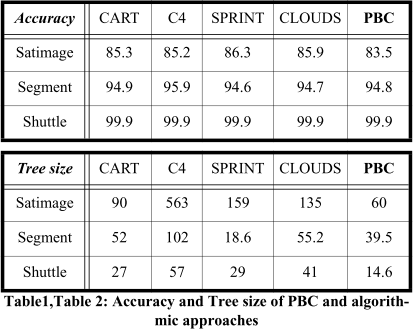
\includegraphics[width=0.75\textwidth]{img/pbc-results.png}
	\end{center}
\end{frame}
% ------------------------------------------------------------------------------
% --------------------------- SLIDE --------------------------------------------
\begin{frame}[allowframebreaks]
	\frametitle<presentation>{Bibliography}
	\bibliographystyle{plain}
	\nocite{Fails2003}
	\nocite{Ankerst1999}
	\nocite{Ware2001}
	\bibliography{bibliography}
\end{frame}
% ------------------------------------------------------------------------------
% --------------------------- SLIDE --------------------------------------------
\begin{frame}
	\begin{center}
		{\Huge QUESTIONS?}
	\end{center}
\end{frame}
% ------------------------------------------------------------------------------
\end{document}
